  \documentclass[12pt]{article}
 
\usepackage[margin=1in]{geometry}
\usepackage{amsmath,amsthm,amssymb}
\usepackage[spanish]{babel}
\decimalpoint
\usepackage[utf8]{inputenc}
\usepackage{enumitem, kantlipsum}
\usepackage{graphicx}
\setlength{\parindent}{0cm} 

\begin{document}
 
\begin{center}
\Large \textbf{C.Física Moderna: Ejercicios Interesantes}\\
\large \textbf{SON OPCIONALES}\\
\end{center}
 
\section{Causalidad} 
 
Suponga que usted es el marco de referencia $S$ y usted ve que un evento $A$ ocurre antes que un evento $B$. Usted mide y estos eventos están separados por un tiempo $\Delta t_{AB}$ y una distancia $\Delta x_{AB}$. Suponga que ambos eventos ocurren sobre el eje $x$(es decir, olvídese de $y$ y $z$).

\begin{enumerate}
	\item Encuentre las condiciones que deben satisfacer $\Delta t_{AB}$ y $\Delta x_{AB}$ de tal forma que el evento $A$ ocurre primero que el evento $B$ sin importar el marco de referencia inercial desde el que se observan los eventos.
	\item Ahora considere un marco de referencia $S'$, que se mueve con velocidad $\vec{v} = v \hat{x}$ relativa a $S$. Determine que sería necesario para que ambos eventos sean simultáneos en el marco $S'$. Por simultaneo se entiende que ocurren al mismo tiempo medido en $S'$.
	\item Nuevamente tiene un marco de referencia $S'$, que se mueve con velocidad $\vec{v} = v \hat{x}$ relativa a $S$. Determine las condiciones en las que ambos eventos ocurren en el mismo punto para $S'$. 
\end{enumerate}
 

 \section{Paradoja de la lanza y el granero} 
 

 
 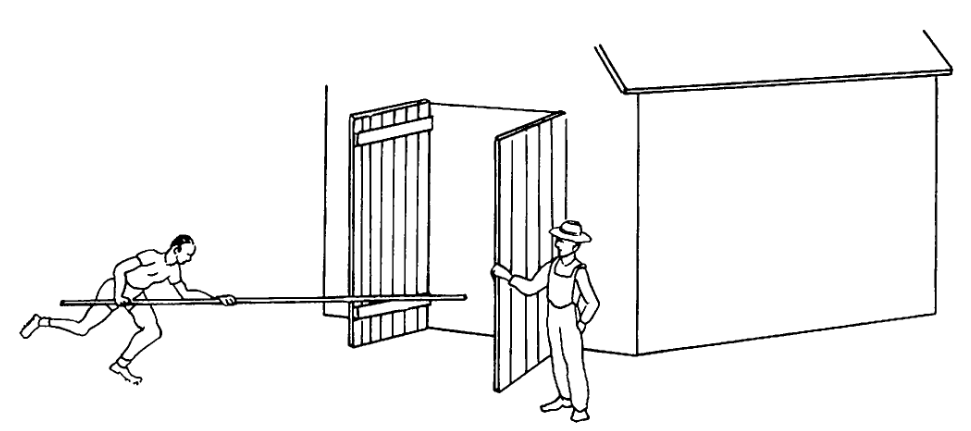
\includegraphics[height=7.4cm]{1}
 
 Rafael tiene una lanza de longitud propia $l_0$ y  un granjero tiene un granero de longitud propia $3 l_0/4$. El granjero le apuesta a Rafael que puede cerrar la puerta de su granero con la lanza de Rafael completamente contenida en su granero. Rafael acepta la apuesta y el granjero le pide a Rafael que corra y  cruce el granero con su lanza a una rapidez de $v = c \sqrt{3}/2$. En esta situación el granjero ve la lanza contraída a una longitud $l_0/2$, por lo que la lanza cabe sin problemas en el granero. El cierra la puerta apenas ve que la lanza está contenida en el interior del granero y le reclama a Rafael su premio. Sin embargo Rafael esta en desacuerdo, para él, el granero se ve contraído a la mitad de su longitud por lo que la lanza no pudo estar contenida en el granero.\\
 
  
 ¿Cómo resolvería usted esta discusión? ¿Se puede decir que la contracción de Lorentz es ''real'' en esta situación?\\

\textbf{Ejercicio del libro ''AN INTRODUCTION TO MECHANICS'' de Kleppner \& Kolenkow}
\end{document}